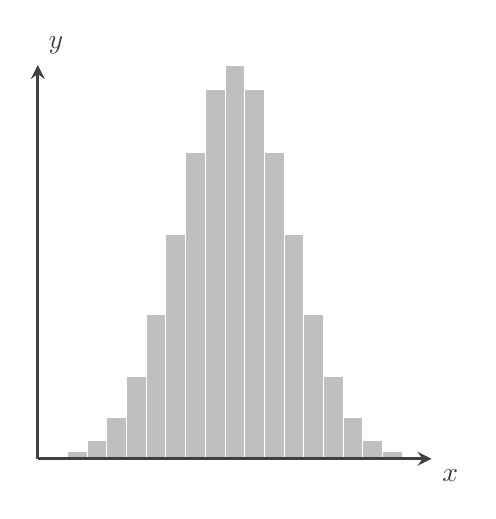
\begin{tikzpicture}[
    declare function={fone(\x)=5*exp(-(\x-2.5)^2);}, 
  very thick, line join=round]

  % Draw squares
  \foreach [evaluate={\x=0.25*\j; \y=fone(\x);}] \j in {0,...,20}{%
    \path [fill=black!25, draw=white, line width=0.2pt] 
    (\x-0.125, 0) -- 
    (\x+0.125, 0) -- 
    (\x+0.125, \y) -- 
    (\x-0.125, \y) -- 
    cycle;
  }

  % Draw functions
%  \draw [black, domain=0.25:4.75, samples=100, variable=\t] 
%  plot (\t, {fone(\t)});

  % x-axis
  \draw [-stealth, black!75] (0,0) -- (5,0) node [below right] {$x$};

  % y-axis
  \draw [-stealth, black!75] (0,0) -- (0,5) node [above right] {$y$};


\end{tikzpicture}
